%%
% このファイルは筑波大学情報学群情報科学類の卒業研究論文のサンプルです. 
% このファイルを書き換えて, このサンプルと同様の書式の論文をLaTeXを使って
% 作成できます. 
% 
% OSやLaTeXの設定によっては漢字コードや改行コードを変更する必要があります. 
%%
\documentclass[a4paper,11pt]{jreport}

%%【PDF, PostScript, JPEG, PNG等の画像の貼り込み】
%% dvipdfmx を使う場合
\usepackage[dvipdfmx]{graphicx}
%% dvipdfmx を使ってPDFの「しおり」を付ける場合
%%\usepackage[dvipdfmx,bookmarks=true,bookmarksnumbered=true,bookmarkstype=toc]{hyperref} \usepackage{pxjahyper}
\usepackage{ulem}
\usepackage{times} % use Times font instead of default one
\usepackage{url}
\usepackage{seqsplit}

\setcounter{tocdepth}{3}
\setcounter{page}{-1}

\setlength{\oddsidemargin}{0.1in}
\setlength{\evensidemargin}{0.1in} 
\setlength{\topmargin}{0in}
\setlength{\textwidth}{6in} 
%\setlength{\textheight}{10.1in}
\setlength{\parskip}{0em}
\setlength{\topsep}{0em}

%% タイトル生成用パッケージ(重要)
\usepackage{coins-jp}

%% タイトル
\title{ユーザ空間並列ファイルシステムのための\\システムコールフックライブラリの設計と評価}
%% 著者
\author{宮内 遥楓}
%% 指導教員
\advisor{建部 修見}

%% 年度と主専攻名
\fiscalyear{2024}
%\majorfield{ソフトウェアサイエンス主専攻}
\majorfield{情報システム主専攻}
%\majorfield{知能情報メディア主専攻}

\begin{document}
\maketitle
\thispagestyle{empty}
\newpage

\thispagestyle{empty}
\vspace*{20pt plus 1fil}
\parindent=1zw
\noindent
%%
%% 論文の要旨
%%
\begin{center}
{\Large \bf 要旨}
\vspace{2cm}
\end{center}
ユーザー空間並列ファイルシステムは, ストレージシステムの性能を向上させるために開発されてきた. 
一方, POSIXインタフェースは, 標準として長い間アプリケーションに使用されてきた.
ユーザ空間ファイルシステム上でアプリケーションを書き換えずに動作させるためにはPOSIXインタフェースへの対応が必要であるが, 
既存手法のFUSEやプリロードライブラリには様々な問題がある.
本研究では, アプリケーションが呼び出すシステムコールをユーザ空間ファイルシステムのAPI呼び出しに置き換えるシステムコールフックライブラリを設計する.
ライブラリの実装においてはバイナリ書き換えに基づくシステムコールフック機構であるzpolineを利用する. 実装したシステムコールフックライブラリ
に対する評価実験の結果, ユーザ空間ファイルシステムのAPIを直接呼び出した場合と比較して性能がほぼ低下しないこと, 既存手法のFUSEを
使用した場合と比較して大幅に性能が向上することを確認した.

%%%%%
\par
\vspace{0pt plus 1fil}
\newpage

\pagenumbering{roman} % I, II, III, IV 
\tableofcontents
\listoffigures
%\listoftables

\pagebreak \setcounter{page}{1}
\pagenumbering{arabic} % 1,2,3

\chapter{序論}
\section{概要}
近年のアプリケーションは, CPUの演算能力がボトルネックとなる演算指向に代わり, データの量や複雑さ, 変化の速度が課題となるデータ指向のものが
多くを占める. スーパコンピュータの主な用途である科学計算シミュレーションやAIにおいても, 膨大な量のデータセットを処理することが要求
されつつある. 一例として, 2020年にOpenAIが発表した言語モデルであるGPT-3は570GB以上のテキストデータを学習データセットとして使用して
いる~\cite{3495883}. CPUやGPUがデータを処理するためにはメモリにデータを載せる必要があるが, メモリの容量以上のデータセットを全部載せる
ことはできないため, 前述のワークロードにおいては何度もストレージからのデータ読み出しを行うことになる. また計算途中の状態をチェックポイント
として記録するため, ストレージへのデータ書き込みも頻発する. そのためストレージ性能の向上はますます重要になる. 

ストレージ性能の向上のために, ファイルシステムの研究が進められている. ファイルシステムはアプリケーションがストレージにアクセスする際の
インタフェースであり, ファイルシステムの設計を工夫することでストレージ性能の向上を図ろうとしている.  

新しく提案されるファイルシステムの多くがユーザ空間で実装されている. ユーザ空間ファイルシステムをアプリケーションから利用するには, 
ファイルシステムAPIの直接呼び出し, FUSE, プリロードライブラリの利用の3つの方法がある. このうちファイルシステムAPIの直接呼び出しに
ついては, アプリケーションのソースコードの変更と再コンパイルが必要になり, ソースコードが手に入らないアプリケーションを動かすことが
できない. もしソースコードがあったとしても, ファイルシステムごとに独自のAPIの仕様を把握し, 適切にAPIを呼び出すよう変更を加えるのは容易
ではない. 現在主流となっているのがFUSEである. FUSEを利用することでユーザ空間ファイルシステムを手軽にマウントすることができ, 通常の
ファイルシステムと同じようにアプリケーションからI/O操作を実行できる. しかしFUSEは設計上ストレージ性能の低下を避けられないため, 
演算性能だけでなくストレージ性能も重要になるHPCアプリケーションではあまり利用されない. 

そこで本研究ではプリロードライブラリの設計を提案する. プリロードライブラリは, \seqsplit{LD\_PRELOAD}環境変数を利用してアプリケーション実行時に
読み込まれることで, 通常のファイルシステムと同じようにアプリケーションからI/O操作を実行できることを目的としている. いくつかのユーザ
空間ファイルシステムでは既にプリロードライブラリを提供しており, 標準ライブラリ(glibc)、または標準ライブラリ内システムコールのI/O関連の関数を
ファイルシステムAPI呼び出しに置き換えている. I/O関連の関数を完全にファイルシステムAPI呼び出しに置き換えられることができれば, 
ファイルシステムAPIの直接呼び出しとほぼ同等のパフォーマンスを実現することができる. しかし既存のプリロードライブラリはI/O関連の関数の
完全な置き換えには至っておらず, アプリケーションによっては実行できない. この問題を解決するため, 全てのシステムコールをファイルシステムAPI
呼び出しに置き換えるシステムコールフックライブラリを本研究で提案・実装する.

\section{本稿の構成}
本稿の構成は以下のとおりである. 第2章では, 本研究の背景について述べ, 提案手法の理解のために重要であるユーザ空間ファイルシステムについて
解説する. 第3章では, アプリケーションがユーザ空間ファイルシステムを利用するための既存の手法について整理する. 第4章では, 提案手法
の設計と実装について説明する. 第5章では, 提案手法の評価実験とその結果について述べる. 第6章では, 評価実験の結果を踏まえた提案手法の考察と
今後の展望をまとめる.
\chapter{背景}

\section{ファイルシステム}
ファイルシステムは, アプリケーションがデータにアクセスするための共通のインタフェースである.

アプリケーションがファイルシステムを利用するときの流れを, \figurename~\ref{fig:Filesystem}を用いて説明する. 
アプリケーションがファイルを開くとき, Linux標準ライブラリ(libc)のopen関数を実行する. open関数はopenシステムコールのラッパー関数であり,
実行するといくつかの前処理を行った後にopenシステムコールを呼び出す. 
ここでシステムコールはアプリケーションがカーネル空間のリソース(メモリ, ストレージ)にアクセスするための手段で, 呼び出されると割り込み
が発生し, カーネル空間に制御が移る.
カーネル空間に制御が移ると, VFS(Virtual File System)によって実際のファイルシステムへのファイルオープン要求に変換される.
VFSは複数のファイルシステムを共存させるためのインタフェースで, これによりファイルシステムごとの細かな違いを意識することなく共通の方法で
ファイルやディレクトリに対する基本的な操作を行うことができる. VFSによって適切なファイルシステムドライバにファイルオープン要求が送られ,
実際のストレージへのアクセスが行われる. 

\begin{figure}[h]
	\begin{minipage}[b]{1\columnwidth}
		\centering
		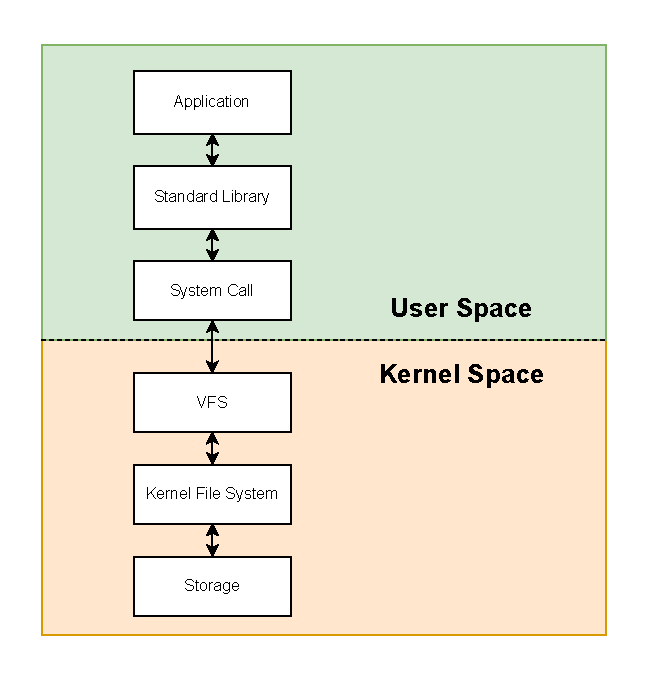
\includegraphics[width=0.9\linewidth]{./figure/filesystem.pdf}
		\caption{ファイルシステム概念図}
		\label{fig:Filesystem}
	\end{minipage}
\end{figure}

\section{ユーザ空間ファイルシステム}
従来, ファイルシステムはカーネルコードの書き換えやカーネルモジュールの追加によってOSカーネル内に実装されてきた. しかし
ファイルシステムの複雑性は年々増しており,Linux 3.6では70以上のファイルシステムのために、全カーネルコード(アーキテクチャ固有の
コードとドライバを除く)のほぼ30\%を占めている~\cite{190583}.
カーネルコードにバグがあった場合, データの破損や脆弱性など様々な問題を引き起こす可能性があるが, 年々複雑になるファイルシステムを
保守し続けるのは容易ではない. 
そこでファイルシステムをカーネル内で実装するのではなく, ユーザ空間上のプロセスとして動作するファイルシステムを開発
することで, この問題を回避することができる. 

ユーザ空間でファイルシステムを開発する利点として, 開発の容易さ, 信頼性, 移植性, パフォーマンスがあげられる. 
ユーザ空間でバグが発生してもシステム全体をクラッシュさせたり破壊したりすることがなく, 開発者にとって安全性が高い. また, カーネル開発が
通常CまたはC++に限定されるのに対し, ユーザ空間では任意のプログラミング言語を使用できる. さらに, カーネルで実行されるコードを減らすことで, 
カーネルのバグが本番システム全体をクラッシュさせる可能性を減らすことにも繋がる. このほか, ユーザ空間のファイルシステムを他のOSに移植するのは
カーネルコードよりも簡単に行うことが可能である. パフォーマンスの面においても, ユーザ空間でより効率的なアルゴリズムを実装した
新しいライブラリを使用できる. 

またファイルシステムをユーザ空間で提供することは, 開発者だけでなくユーザにもメリットがある. ファイルシステムの中には特定の
アプリケーションに特化したものがあり, それらのファイルシステムをアプリケーションから利用できれば大幅な性能向上につながる可能性がある. 
しかしファイルシステムの追加はカーネルの変更に当たるため, 特に複数人が利用する計算機システムにおいて, 自由にファイルシステムを追加すること
はできない. 
対してユーザ空間ファイルシステムであればカーネルの変更なくアプリケーションから利用することができるため, 画期的な実装のファイルシステムを
試すことが容易に可能である. 

このような背景から, 多くの新しいファイルシステムがユーザ空間で開発されるようになった.
特に, 産業や学術研究において, ファイルシステム設計の新しいアプローチのプロトタイプ作成や評価を迅速に行うために, ファイルシステムが
ユーザ空間で開発されている. 
またカーネルの機能のうち, プロセス管理, スケジューラ, メモリ管理といった必要最低限の機能を実装するマイクロカーネルアーキテクチャでは, 
ファイルシステムをユーザ空間で提供する仕組みが採用されている. 
\section{並列ファイルシステム}
HPCアプリケーションは計算の高速化のため並列化を行うことが多く, その際のデータ読み出しで多数のI/Oリクエストが発生する. 通常の
ファイルシステムでは1つのサーバがリクエストに対応するが, リクエストの量によっては対応しきれずボトルネックの原因になる. そこで複数の
サーバ, または複数のストレージを仮想的に1つのストレージとして扱えるようすることで高いストレージ性能を達成する並列ファイルシステムがHPC
分野ではよく使用される. 


\chapter{既存手法}
アプリケーションの書き換えなしにユーザ空間ファイルシステムを利用する方法は大きく分けて2つある.
\section{FUSE}
FUSE(Filesystem in Userspace)はユーザ空間ファイルシステムを開発するときに最も使用されているフレームワークである. FUSEを利用することで
容易にユーザ空間ファイルシステムをPOSIXインターフェースに対応させることができるため, SSHFS~\cite{hoskins2006sshfs}, GlusterFS~\cite{davies2013scale}, 
ZFS~\cite{rodeh2003zfs}など数多くのFUSEベースのファイルシステムが開発されており, その数は100を超える.

アプリケーションがFUSEを介してユーザ空間ファイルシステムにアクセスする過程を\figurename~\ref{fig:FUSE}に示す. アプリケーションが
標準ライブラリを通じてシステムコールを発行し, VFSに到達するまでは通常のファイルシステムアクセスと同じである. VFSにはFUSEドライバが
登録されており, このドライバとユーザ空間ファイルシステムが/dev/fuseブロックデバイスを介してやり取りをする.

この仕組みによりカーネルに変更を加えることなくファイルシステムを追加することができる. 
しかしながら,アプリケーションとFUSEプロセスとの通信コストや,コンテキストスイッチによるオーバーヘッドが原因の性能低下により, 
特にパフォーマンスが求められるHPC分野での利用は適していないと論じられている~\cite{brinkmann2020ad}. そのためFUSEから派生した
より効率的なユーザ空間ファイルシステムフレームワークの研究も多くされている~\cite{294791, zhu2018direct, 3494556}. 

\newpage


\begin{figure}[h]
	\begin{minipage}[b]{1\columnwidth}
		\centering
		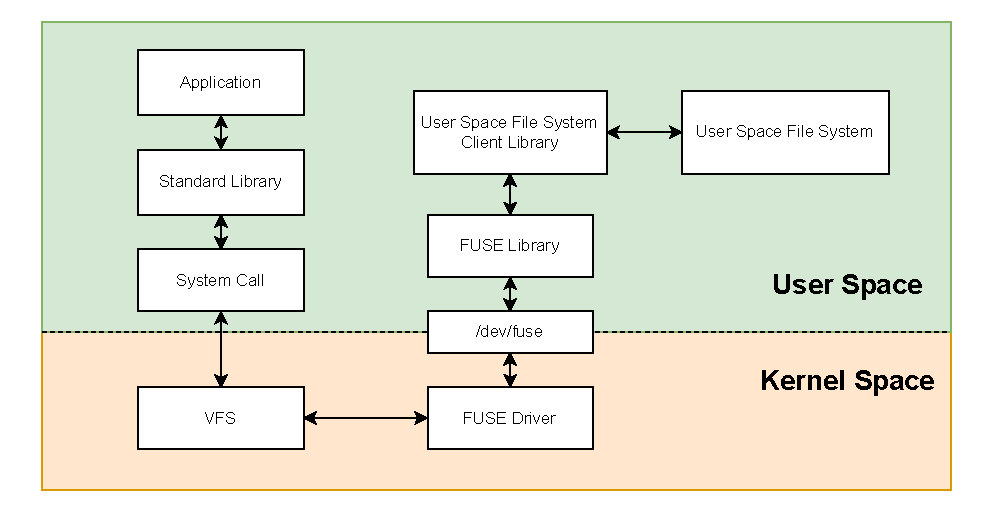
\includegraphics[width=0.9\linewidth]{./figure/FUSE.pdf}
		\caption{FUSE アーキテクチャ}
		\label{fig:FUSE}
	\end{minipage}
\end{figure}

\newpage


\section{プリロードライブラリ}
Linuxには共有ライブラリの関数をフックできるLD\_PRELOAD環境変数が存在する. \seqsplit{LD\_PRELOAD}に共有ライブラリのパスを
指定すると, プログラム起動時に動的リンカが対象ライブラリを優先的にリンクする. これにより, ある関数がLD\_PRELOADに指定したライブラリに
存在する場合, 他のライブラリの実装より優先して呼び出されるため, 既存関数の実装差し替えや, main関数実行前に任意の関数を実行することが
可能になる. 各ユーザ空間ファイルシステムが提供するプリロードライブラリをLD\_PRELOADで指定してアプリケーションを実行することで, 
ソースコードの変更や再コンパイルなしにユーザ空間ファイルシステムを利用することが可能になる. しかしアプリケーションが呼び出すI/O関数
を網羅的にフックすることは容易ではないため, プリロードライブラリの作成には次に示すライブラリが使用されることが多い. 

Gotcha~\cite{gotcha}は任意の関数をラップするライブラリで, LD\_PRELOADに似ているが, プログラム可能なAPIを介して動作する. 
UnifyFS~\cite{10177390}はGotchaを利用してlibc(C標準ライブラリ)のI/O関連の関数をフックし, UnifyFSのAPIに置き換えることで
POSIXインタフェースの対応を行っている.

syscall\_intercept~\cite{syscall-intercept}は, メモリにロードされたglibcのテキストセグメント中のsyscall命令を検知し, jmp命令に
置き換えることで任意の関数呼び出しを可能にするライブラリである.
syscall\_interceptを使用してPOSIXインタフェース対応をしているユーザ空間ファイルシステムにはGekkoFS~\cite{8514892}がある.
glibcの関数をフックする場合と比較して, 少数のシステムコールフックを定義するだけで済むため, ファイルシステムが提供する
プリロードライブラリの実装は相対的に容易である. しかしsyscall\_interceptはLinuxのglibcにしか対応していないため, glibcを使わない
アプリケーションは動かない可能性がある.

\chapter{提案手法}
本研究では, ユーザ空間ファイルシステムにおけるPOSIXインタフェース対応のために, 前章で既存手法として挙げたプリロードライブラリの新しい
設計を提案する. 具体的には, ユーザ空間ファイルシステム上で動作するアプリケーションによって呼び出されるシステムコールをフックする
ライブラリを設計する. また提案手法の評価のため, ユーザ空間並列ファイルシステムであるCHFS~\cite{tatebe2022chfs}のPOSIX
インタフェース対応を目的としたシステムコールフックライブラリを実装する. ライブラリの実装においては, システムコールフックメカニズムの
zpoline~\cite{288689}を利用する.


\section{システムコールフックライブラリの設計}
システムコールフックライブラリの設計を\figurename~\ref{fig:Syscall hook}を用いて説明する.
アプリケーションがユーザ空間ファイルシステムにアクセスするエントリポイントとして, 仮想的なマウントポイント/virtual\_mount\_point を
仮定する. アプリケーションから呼び出されたシステムコールに含まれるパス名が/virtual\_mount\_point で始まる場合, そのファイルはユーザ
空間ファイルシステムの管理下にあると判断し, システムコールの呼び出しをユーザ空間ファイルシステムのクライアントライブラリのAPI呼び出し
に置き換える. そうでない場合は本来のシステムコールを呼び, 通常通りVFSを経由してカーネル空間のファイルシステムにアクセスする.

システムコールがフックされた場合, 本来のシステムコールは呼ばれないためコンテキストスイッチが発生しない. そのためFUSEで発生している
ようなコンテキストスイッチに起因するオーバヘッドを削減することができ, ユーザ空間ファイルシステムを効率的に利用することが可能になる.

\begin{figure}[h]
	\begin{minipage}[b]{1\columnwidth}
		\centering
		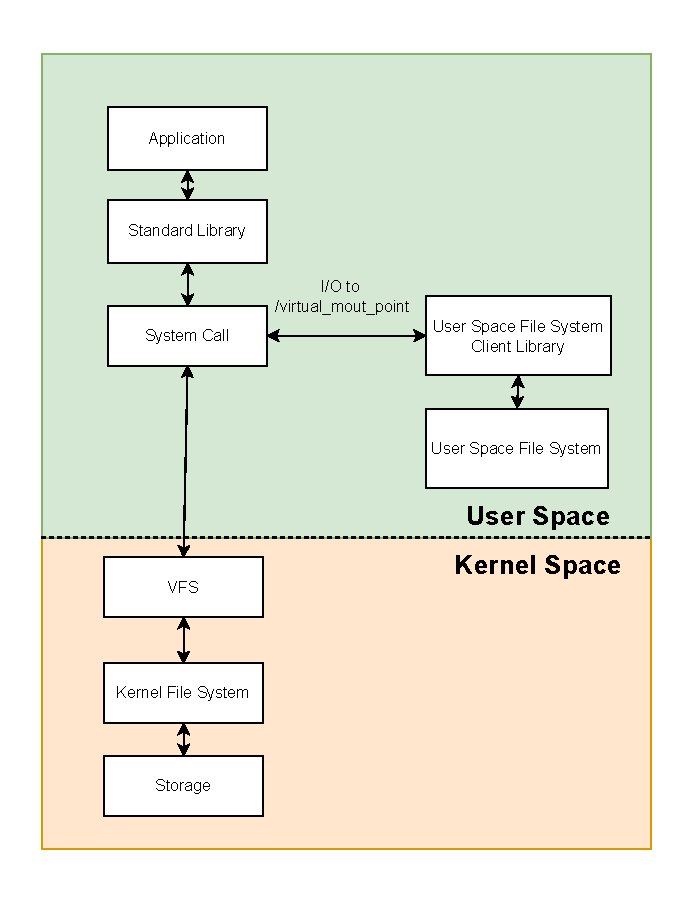
\includegraphics[width=0.9\linewidth]{./figure/syscall_hook_v2.pdf}
		\caption{システムコールフックによるファイルシステムアクセス}
		\label{fig:Syscall hook}
	\end{minipage}
\end{figure}

\section{zpoline}
zpolineは安形らによって提案された, システムコールを高速にフックする手法である. 既存手法で例に挙げたsyscall\_interceptにはglibc内で
呼び出されるシステムコールしかフックできないという問題があったが, zpolineではバイナリ書き換えとトランポリンコードを組み合わせることで
この問題を解決し, 全てのシステムコールをフックすることを可能にした.

zpolineがシステムコールをフックする仕組みを\figurename~\ref{fig:Zpoline mechanism}を用いて説明する. zpolineは\seqsplit{LD\_PRELOAD}
でロードされることを想定したライブラリとして実装されており, アプリケーションのmain関数が実行されるよりも前にシステムコールフックの
準備を行う. 

プログラムのバイナリがメモリにロードされると, zpolineはまずロードされたバイナリの書き換えを実行する. ユーザ空間プログラムが
カーネルの機能を利用する際には必ずシステムコールを発行する必要がある. そのために使われる syscall / sysenter 命令は2byteの機械語
命令であり, システムコールを他の関数呼び出しに置き換えるには syscall / sysenter 命令を別の機械語命令に書き換えてやればよい. しかし
3byte以上の機械語命令で書き換えてしまうと syscall / sysenter 命令の次の命令を上書きしてしまい, プログラムが正常に動作しなくなるため, 
2byteという非常に厳しい制約のもと命令を書き換える必要がある. zpolineは callq *\%rax という2byteの命令で syscall / sysenter 命令を
書き換える. callq *\%rax は\%raxレジスタに入ったアドレスにジャンプし, ジャンプ元のアドレスをスタックへプッシュするという命令である. 
ここでLinuxのシステムコールの呼出規約では\%raxレジスタにシステムコール番号を入れておく必要がある. システムコール番号はカーネルの定義
により高々500に収まる数のため, callq *\%rax が実行されるとアドレス0 \textasciitilde 500にジャンプする.

次にzpolineはメモリアドレス0から最大のシステムコール番号+1の位置に, トランポリンコードと呼ばれる任意のフック関数にジャンプするための
コードを用意する. まずメモリアドレス0から最大のシステムコール番号までをnop命令で埋める. nop命令は何もせず次の命令を実行する命令である.
その後最後のnop命令の次の位置に, 任意のフック関数があるアドレスにジャンプするためのコードを埋め込む.

zpolineによるシステムコールフックの準備が完了すると, 通常通りプログラムのmain関数が実行される. プログラム内でシステムコールが呼ばれると, 
バイナリ書き換えにより syscall / sysenter 命令から置き換えられた callq *\%rax 命令が実行される. callq *\%rax 命令によりメモリ上では
システムコール番号のアドレスに移動する. 移動先はトランポリンコードの設置によりnop命令で埋められており, nop命令が繰り返し実行された後, 
任意のシステムコールフック関数があるアドレスにジャンプする. これによりシステムコールに対し任意の関数呼び出しが実行される.



\begin{figure}[h]
	\begin{minipage}[b]{1\columnwidth}
		\centering
		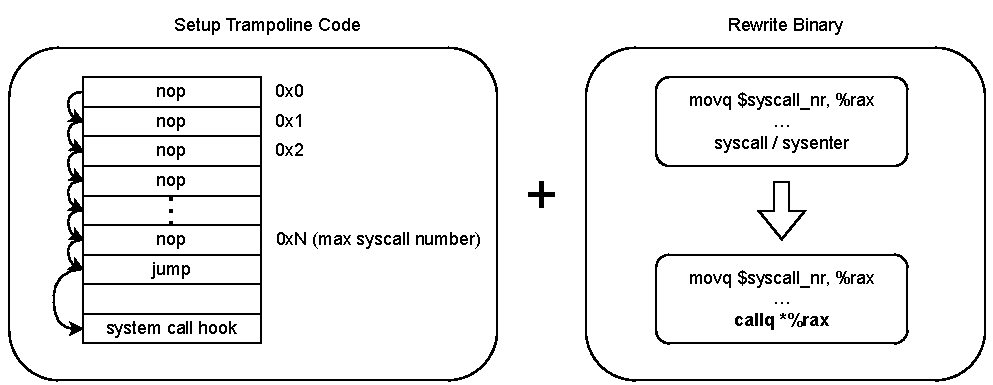
\includegraphics[width=0.9\linewidth]{./figure/zpoline_mechanism.pdf}
		\caption{zpoline メカニズム}
		\label{fig:Zpoline mechanism}
	\end{minipage}
\end{figure}

\section{CHFS}
CHFSは建部らの開発するスーパコンピュータ向けの並列ファイルシステムである. 近年のスーパコンピュータは各計算ノードにローカルストレージを
持つことが多く, CHFSはそれらのストレージをまとめて1つのストレージであるかのように扱えることを目的としている. CHFSはスーパコンピュータ
向けのI/O性能の世界ランキングIO500の2023年6月の10ノード研究部門において21位を記録しており, 高性能計算分野における今後の利用が期待される.

しかしながらIO500で示されたCHFSの性能は, ベンチマークプログラムのファイルI/O部分の関数をCHFSのAPIに置き換えて実行することで測定された
ものであり, 実際のアプリケーションの複雑なソースコードを同様に書き換えることは現実的ではない. そのためアプリケーションをCHFS上で
動作させるにはFUSEを利用したマウントが必要になるが, 前章で述べた通り通信コストやコンテキストスイッチによる性能低下が予想される.

本研究では提案した設計に基づき, CHFSのシステムコールフックライブラリを実装する. /chfs を仮想的なマウントディレクトリと設定し, /chfs
から始まるパス名を対象とするシステムコールを, zpolineを利用してCHFSのAPI呼び出しに置き換える. 次章の実験ではIO500で使用されるベンチ
マークプログラムであるIOR~\cite{ior}を用いて性能評価を行う. IORベンチマークが呼び出すシステムコールに対応するため, 実装する
ライブラリではread, write, open, close, stat, lstat, lseek, pread64, pwrite64, openat, fsync, newfstatat システムコールを
フックする.

\chapter{評価実験}
前章で実装したシステムコールフックライブラリの評価実験を行う. 本実験の目的としては, ユーザ空間ファイルシステムが提供する
クライアントライブラリを使用した場合と比べてどの程度ストレージアクセス性能が保たれるか評価すること, また既存手法の中で
最もよく用いられるFUSEとの性能を比較することである. 

\section{実験環境}
実験環境として筑波大学計算科学研究センターが運用するPegasusスーパーコンピュータを利用する. Pegasusは各計算ノードに専用のストレージを
保持しており, NVMe SSDとIntel Optane Persistent Memory(PMEM)を利用できる.  計算ノード間はInfiniBand NDR 200で接続されており, 
帯域幅は200Gbpsである. 
\section{予備実験: FUSE性能評価}
最初に予備実験として, 既存手法であるFUSEを利用した際のストレージ性能の低下がどの程度発生するかを調査する. 予備実験ではPegasusシステム
の計算ノードを1台使用し, ローカルのSSDを使用する. ローカルSSDには, /scrとしてマウントされているXFSファイルシステムを通じてアクセスできる.
/scrに直接ファイル読み書きを実行した場合と, ファイル読み書きの要求をそのまま/scrに流すだけのダミーのファイルシステムをFUSEを使用して
マウントし, ファイル読み書きを実行した場合の性能をIORベンチマークを使用して比較する. IORはプロセス数を1, file-per-process方式で実行
する. 

実験結果を\figurename~\ref{fig:FUSE Performance}に示す. FUSEを利用した帯域幅性能は, 直接読み書きした場合に比べ, 読み込み性能が
1/7, 書き込み性能が1/3という結果になった. 

\newpage

\begin{figure}[h]
	\begin{minipage}[b]{1\columnwidth}
		\centering
		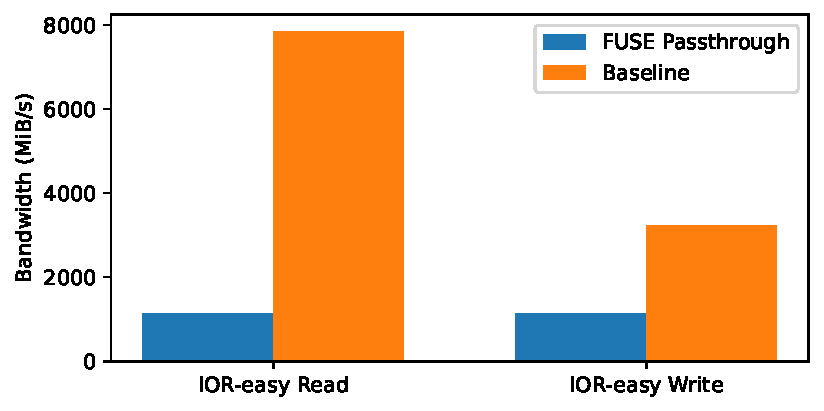
\includegraphics[width=0.9\linewidth]{./figure/fuse_overhead.ssd.pdf}
		\caption{ネイティブファイルシステムとFUSEの性能比較}
		\label{fig:FUSE Performance}
	\end{minipage}
\end{figure}
\section{実験方法}
本実験ではIORベンチマークを実行してCHFSに対するファイル読み込み/書き込み帯域幅を測定する. 提案手法を含む
以下の3種類の条件下でベンチマークを実行し, その性能を比較する. 

\subsection{ネイティブAPI}
ファイルシステムが提供するクライアントライブラリのAPIを利用してファイルにアクセスする. 本実験ではIORベンチマークのソースコードを変更し, 
CHFSクライアントライブラリの関数を呼び出すことでCHFS上のファイルへの読み書きを行う. 
\subsection{FUSE}
CHFSサーバを起動した後, chfuseコマンドを使用して指定のディレクトリにマウントする. IORベンチマークのファイル読み込み・書き込みは
マウントしたディレクトリに対して実行する. 
\subsection{システムコールフック(提案手法)}
前章で実装したシステムコールフックライブラリを利用する. 仮想的なマウントディレクトリ/chfsに対してIORベンチマークのファイル読み込み・
書き込みを行う. 
\section{実験設定}
Pegasusシステムにおいて, 計算ノード10台をCHFSサーバとして割り当て, さらに1台をIORベンチマークの実行に使用し, 合計で11台の計算ノードを
専有する. 各計算ノードに設置されているPMEMをdevdaxモードで使用する. 

CHFSはチャンクサイズを16MiBに設定し, 各ノード46プロセスでCHFSサーバを起動する. 通信プロトコルにverbs, バックエンドにpmemkvを利用する. 

IORはプロセス数を1, 2, 4, …と16まで増やしながら実行する. IORではfile-per-process方式でアクセスし, 各プロセスが別々のファイルに
対して1TiB読み書きする. この操作を5回行い, 帯域幅の平均を求める. 
\section{結果}

実験結果を\figurename~\ref{fig:Evaluation read}と\figurename~\ref{fig:Evaluation write}に示す. どの条件でもプロセス数を増やすに
つれ帯域幅が増加していることがわかる. 読み込みの16プロセスにおいて性能の増加がないのは, Pegasus計算ノード間の通信帯域幅200Gbpsに
到達していると考えられる. 

基準であるネイティブAPIを使用した場合の性能に対して, 提案手法のシステムコールフックは読み込み・書き込みともに同程度の性能を示した. 
またFUSEを使用した場合と比較して提案手法は5.3倍から6.4倍高い性能を示した. 

\newpage

\begin{figure}[h]
	\begin{minipage}[b]{1\columnwidth}
		\centering
		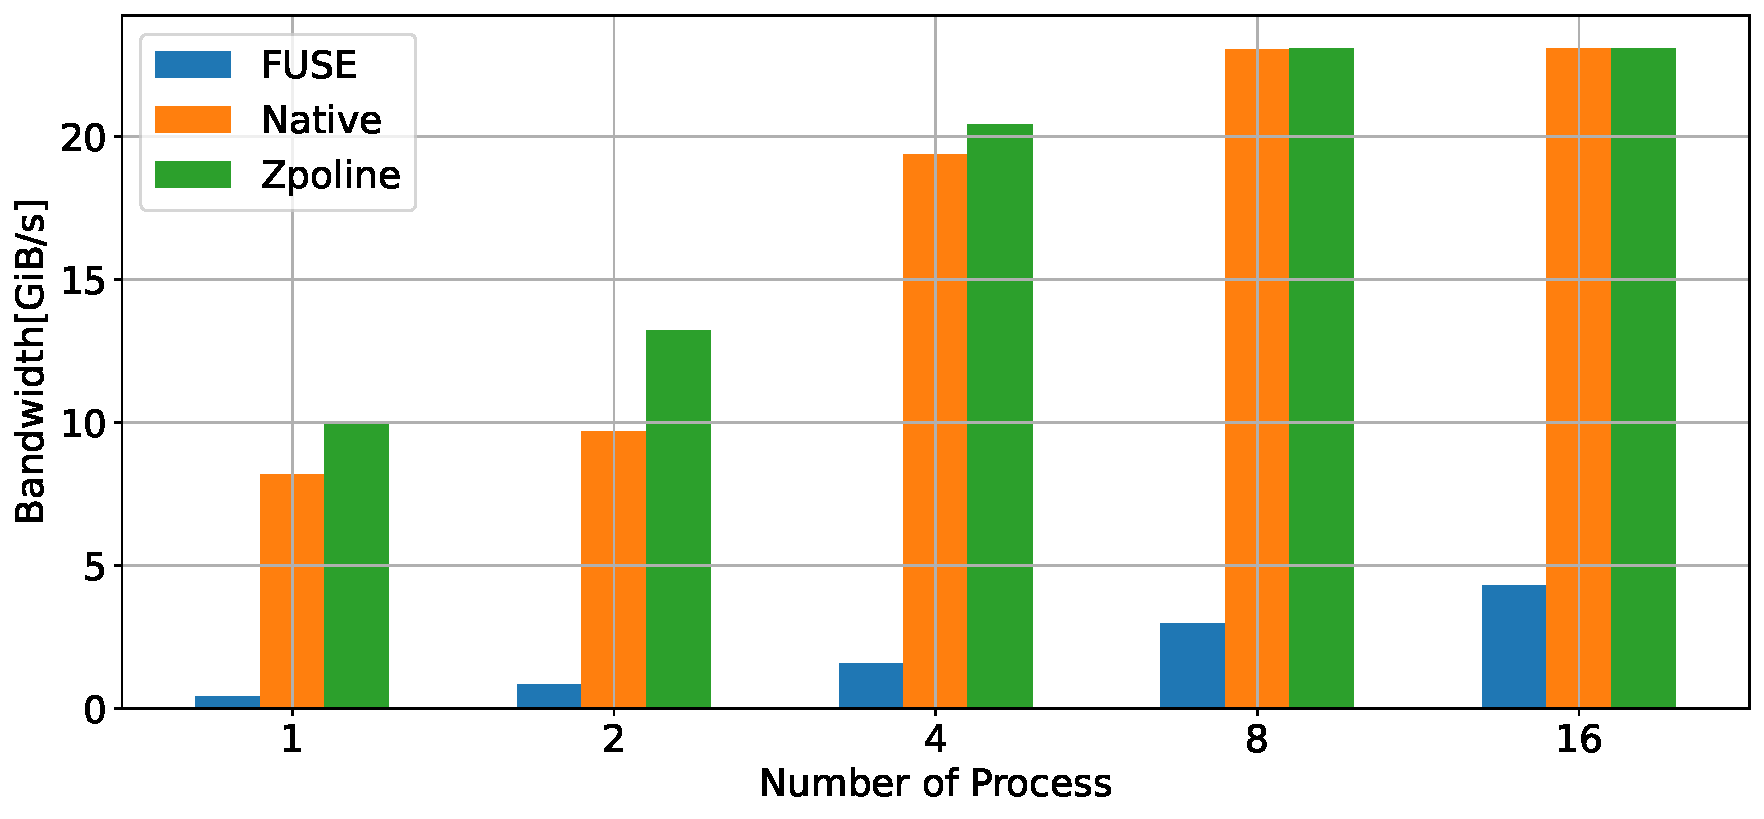
\includegraphics[width=0.9\linewidth]{./figure/ior_benchmark_read.pdf}
		\caption{IOR 読込み性能}
		\label{fig:Evaluation read}
	\end{minipage}
\end{figure}

\begin{figure}[h]
    \begin{minipage}[b]{1\columnwidth}
		\centering
		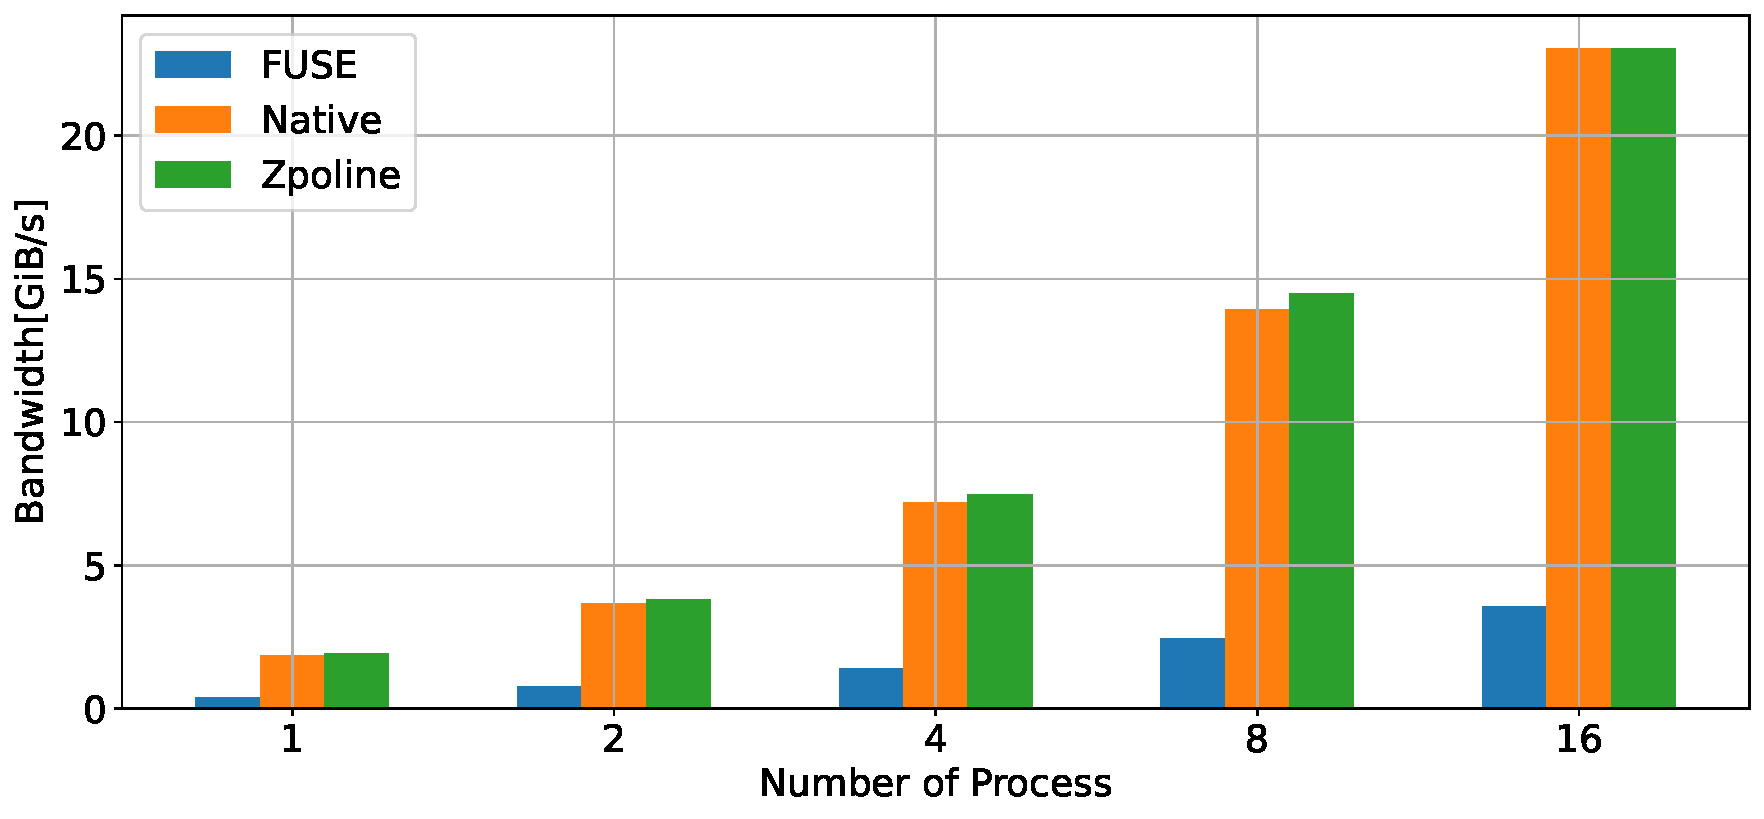
\includegraphics[width=0.9\linewidth]{./figure/ior_benchmark_write.pdf}
		\caption{IOR 書込み性能}
		\label{fig:Evaluation write}
	\end{minipage}
\end{figure}

\chapter{終論}
\section{まとめ}
ユーザ空間ファイルシステムのPOSIXインタフェース対応を目的とした手法はいくつか存在するが, 既存手法には性能や汎用性の面で問題があった.
本研究ではファイル操作に必要なシステムコールをユーザ空間ファイルシステムのAPIに置き換える, システムコールフックライブラリを設計した.
高速なシステムコールフック機構であるzpolineを使用したシステムコールフックライブラリを実装し, 性能評価を行った. 性能評価においては
ストレージ性能を評価するIORベンチマークを用いて評価を行い, ユーザ空間ファイルシステムのAPIを直接呼び出した場合と比較してほぼ性能が
低下しないこと, 既存手法のFUSEを利用した場合と比較して5.3倍から6.4倍高い性能を示すことを確認した.

\section{今後の展望}
IORベンチマークを用いた性能評価により, 提案手法の有用性を示した. 今後は実アプリケーションの
I/O性能の向上に向け, より多くの実アプリケーションを動作させることを目指す. 実アプリケーションは今回使用したIORベンチマークよりも多くの
システムコールを使用するため, システムコールのフックを増やす必要がある. 現在は
ファイルディスクリプタを複製するdup・dup2, 子プロセスを生成するforkシステムコール等の対応が完了している. その結果, Linuxのls, 
touch等ファイルシステムに関連するコマンドや, 与えられた画像データセットをニューラルネットワークで分類する簡単なPyTorchプログラムを
CHFS上で動作させることに成功している. 

今後はより大規模かつ実際に使用されているものに近いアプリケーションを動作させる. 
第1章で説明したように, 近年の科学計算シミュレーションやAIワークロードでは大量のデータをストレージから読み込む必要があるため, 
CHFSを利用できれば学習をより短時間で完了できる可能性がある. そのため現在は機械学習ワークロード向けのストレージベンチマーク
であるMLPerf Storageベンチマーク~\cite{mlperfstorage}を動作させることを目標にシステムコールのフックを進めている. 

\chapter*{謝辞}
\addcontentsline{toc}{chapter}{\numberline{}謝辞}
1年間親身かつ丁寧に研究を指導してくださった筑波大学計算科学研究センターの建部修見教授に深く感謝申し上げます. 
加えて, 研究テーマの相談段階から論文作成にいたるまで研究にご指導ご尽力いただき, また国際会議の発表において共著者として
ご協力いただいたHPCS研究室の小山創平氏に大変感謝申し上げます. 
また, 計算科学研究センターの研究員である平賀弘平氏, HPCS研究室の杉原航平氏にも研究を進めるうえで多大なアドバイスをいただきました. 感謝申し上げます. 
同時に, 計算科学研究センターの職員の皆様, 特に同センター秘書の桑野洋子氏には事務的な面で研究をサポートしていただきありがとうございました. 
HPCS研究室の皆様には, 研究を進めるにあたり議論を通じてご協力いただきました. 
そして共同研究先である富士通研究所の皆様には学外としての立場から大変ありがたいご支援をいただきました. ありがとうございました. 
最後に, これまで大学生活を共にした友人と, 学生生活を支えてくれた家族に心から感謝致します. 

\newpage

\addcontentsline{toc}{chapter}{\numberline{}参考文献}
\renewcommand{\bibname}{参考文献}

\bibliography{main}
\bibliographystyle{junsrt}

\end{document}
